%Acá explicamos cómo extrajimos los datos, qué características tiene la muestra (muchos de los análisis/gráficos ya los hicimos), cómo la separamos, y qué análisis estadísticos estamos realizando (es la parte que nos falta)


\section{Extracción de Datos}

Para la recolección de tuits, primero se extrajo una cantidad de usuarios con información geográfica disponible con el fin de obtener todos sus tuits.
Los usuarios se buscaron por provincia de modo tal que haya una cantidad aproximadamente equitativa de cada una.
La búsqueda de los usuarios se hizo de la siguiente manera:

Por cada provincia de la Argentina, se extrajo las ubicaciones de cada uno de sus departamentos, de los partidos de la provincia de Buenos Aires y de las comunas de la Ciudad Autónoma de Buenos Aires. El conjunto de estas forman la subdivisión de segundo orden de la república Argentina. La lista de departamentos/partidos/comunas fue extraída a partir de los datos publicados del Censo Argentino del año 2010. Para extraer los tuits se utilizó la librería de \textit{python} llamada \textit{tweepy}.
De esta manera se recolectó aproximadamente 2000 usuarios por provincia, lo que resulta en 46000 usuarios argentinos. Sobre este conjunto de usuarios se buscaron los tuits. Se decidió no tener en cuenta los retuits dado que no son escritos por los usuarios sino que son una mera copia de otros tuits. 


\subsection{Búsqueda geolocalizadas}

Las búsquedas geolocalizadas de la API de \textit{twitter} primero intentan de buscar tuits cuyas coordenadas sean las buscadas. En caso de no tener éxito, buscará aquellos tuits creados por usuarios que tienen en el campo \textit{location} de su perfil un lugar cuyo geocódigo coincida con el de sus coordenadas. Es decir, si se hace una búsqueda inversa de las coordenadas, devuelve el lugar de su perfil.

Una vez obtenida la lista de ubicaciones, se realizaron búsquedas por cada provincia con centro en las coordenadas de los departamentos de la misma y con un radio de 20 millas. Sobre el resultado de esta búsqueda, únicamente se seleccionaron los usuarios que tienen como campo \textit{location} al menos uno de los nombres de las ciudades de la provincia. Con esta precaución eliminamos los posibles tuits de turistas que escribieron en un lugar pero que no viven allí.
/h
En el gráfico de la figura \ref{fig:busqueda_usuarios} se muestran las ubicaciones de los usuarios de la muestra de desarrollo:


\begin{figure}[!ht]\centering
  \begin{minipage}{0.31\textwidth}
    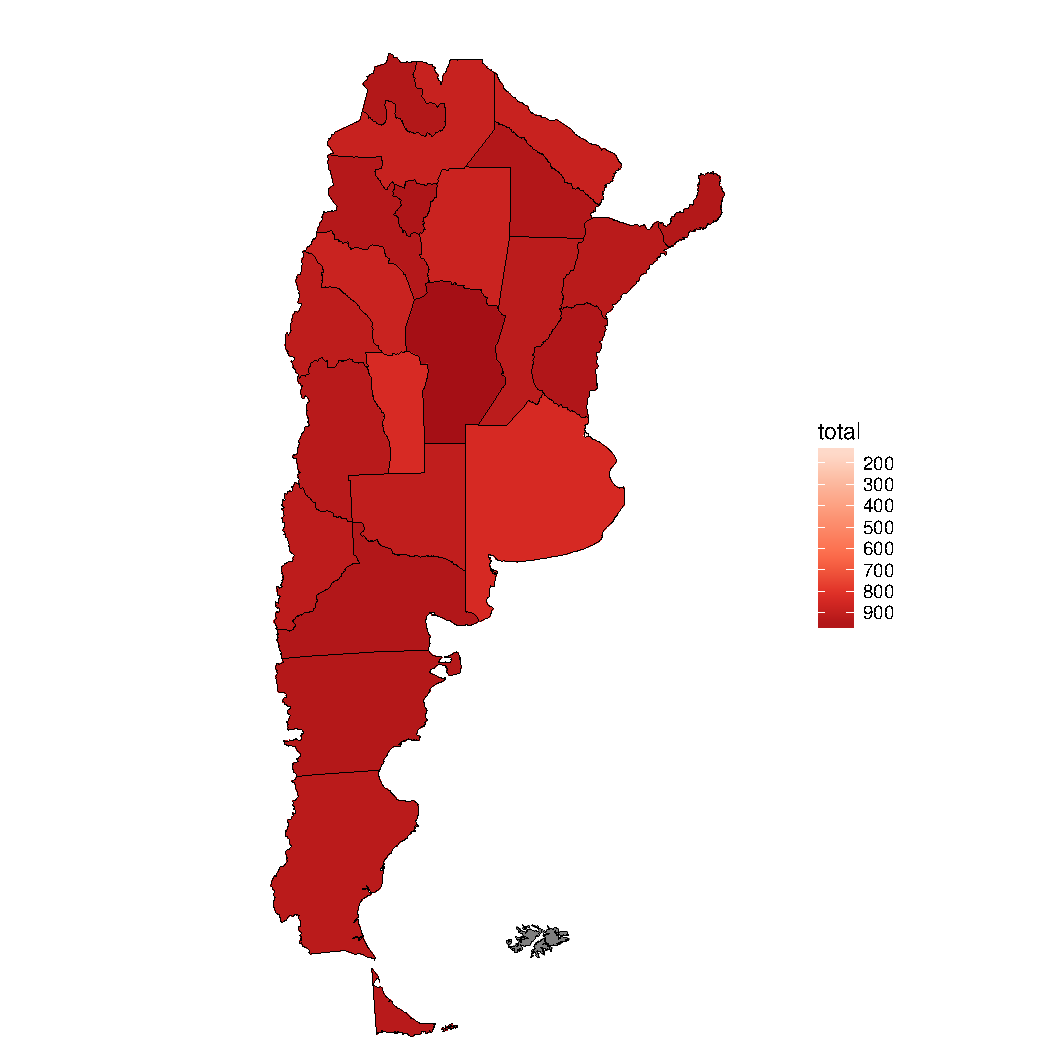
\includegraphics[width=\linewidth]{./images/mapaprovincias.pdf}
    \caption{} 
    \label{fig:mapaProvincias} 
   \end{minipage}
   \begin{minipage}{0.31\textwidth}
    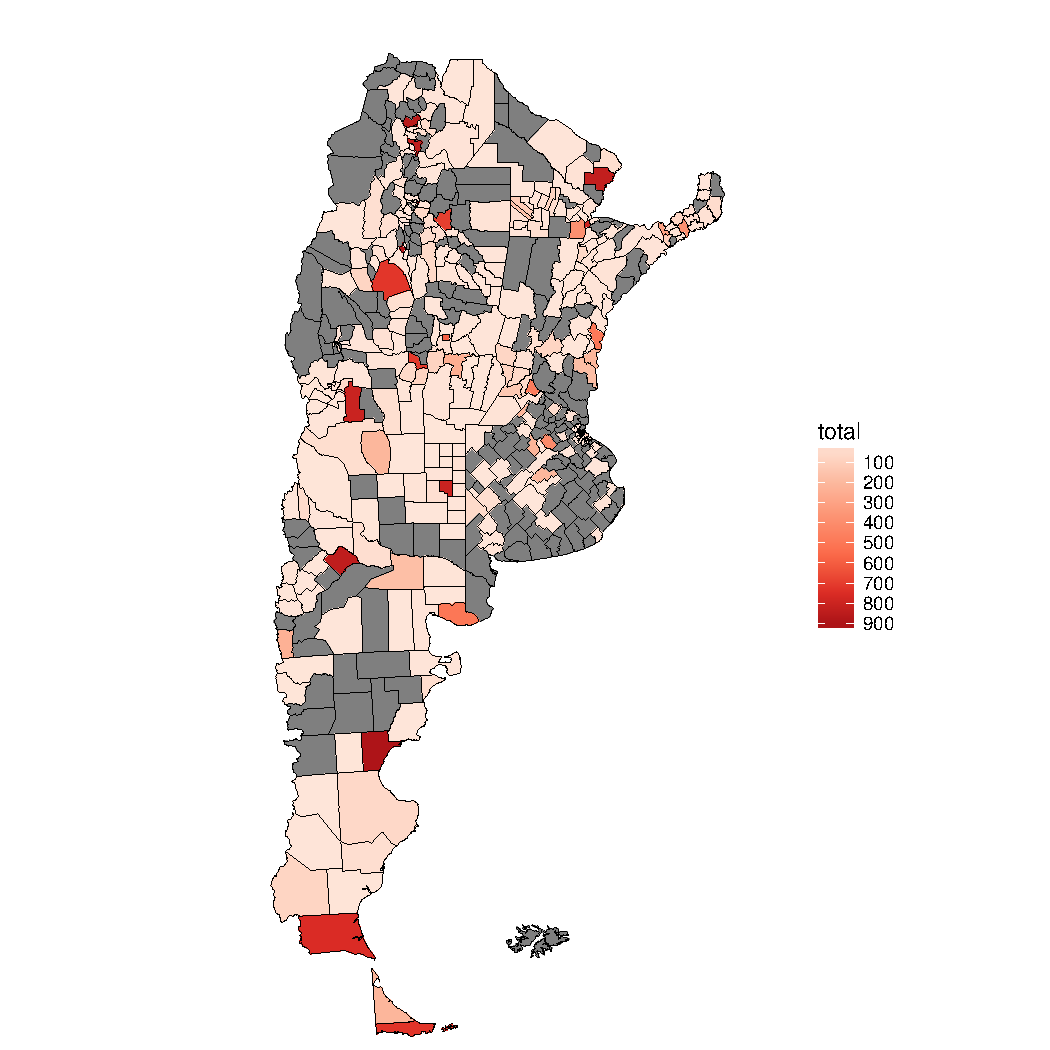
\includegraphics[width=\linewidth]{./images/mapadepartamentos.pdf}
    \caption{} 
    \label{fig:mapaDepartamentos} 
   \end{minipage}
   \begin{minipage}{0.31\textwidth}
    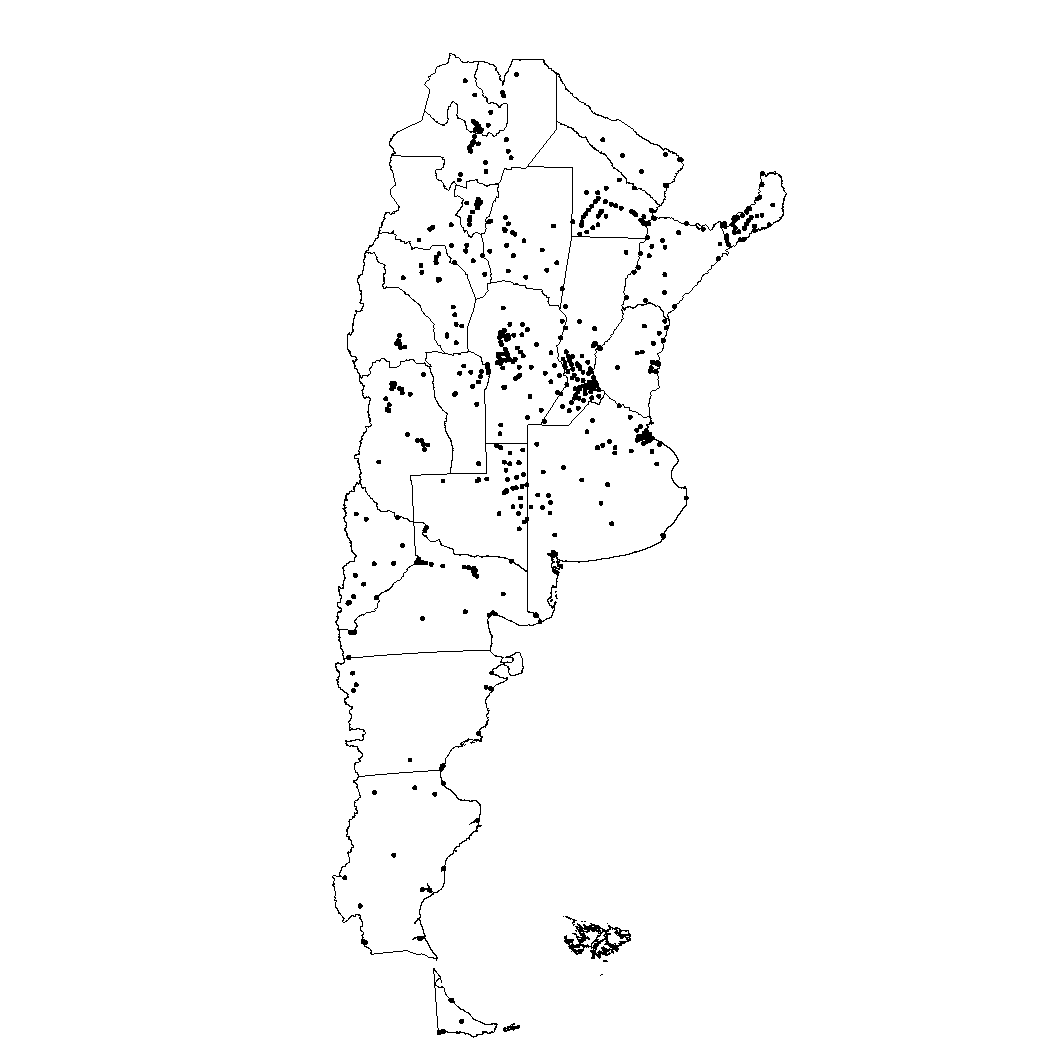
\includegraphics[width=\linewidth]{./images/mapaprovinciasConPuntos.pdf}
    \caption{} 
    \label{fig:mapaPuntos} 
   \end{minipage}
   


   \caption{Ubicaciones de los usuarios: En la figura \ref{fig:mapaProvincias} se muestra un mapa de Argentina con la distribución de los usuarios en las provincias sobre el conjunto de desarrollo. El mapa de la figura \ref{fig:mapaDepartamentos} permite visualizar la distribución de los usuarios en los departamentos sobre el conjunto de desarrollo. Se muestra con áreas grises los departamentos que no poseen usuarios que hayan definido el campo ubicación de su perfil en ese lugar. El mapa \ref{fig:mapaPuntos} muestra la distribución de las coordenadas obtenidas a partir de todos los usuarios del conjunto de desarrollo. Las coordenadas fueron obtenidas a través de un proceso de geocodificación. } 
  \label{fig:busqueda_usuarios} 

\end{figure}

En la figura \ref{fig:mapaProvincias} se ve que la distribución de usuarios en las provincias es bastante pareja. Si bien en la figura \ref{fig:mapaDepartamentos} hay regiones grises que indican la ausencia de usuarios en ese lugar, cabe destacar que los mapas se realizaron obteniendo las coordenadas geográficas a partir de la ubicación definida en el perfil del usuario. Por lo tanto, si una persona declara que vive en \textit{Tucumán, Argentina}, contabilizamos como que esa persona vive en la capital de esa provincia, lo cual puede no ser cierto. Sin embargo, esto no invalida los resultados puesto que la granularidad del análisis es a nivel provincial. Finalmente para ver la distribución de las coordenadas de los usuarios a lo largo del país mostramos la figura \ref{fig:mapaPuntos}. Se puede observar que en la mayoría de las grandes ciudades hay usuarios en nuestro conjunto de datos. En el apéndice se puede encontrar un mapa \ref{mapaGPS} donde se contabilizaron todos los tuits con coordenadas geográficas del conjunto de datos. En este gráfico se puede observar que la distribución es mucho más amplia, aunque sigue habiendo más concentración de usuarios en aquellos departamentos con más densidad poblacional.

Si bien en este trabajo nos enfocamos en las coordenadas de las localidades dentro de Argentina, basta con cambiar las coordenadas y los nombres de las localidades que tienen que tener los campos \textit{location} para realizar un análisis sobre otros países en una segunda etapa.


\section{Datos de desarrollo y de validación}

Por cada provincia se tomó a los usuarios de la misma y se los dividió para tener un conjunto de datos de desarrollo y uno de validación. El conjunto de validación fue creado para poder corroborar que los resultados obtenidos por el análisis del conjunto de desarrollo no sean algo intrínseco de esta muestra, sino que se pueden extrapolar a toda la población. 
La división de los datos se realizó de manera tal que los conjuntos resultantes sean lo más independientes posibles: 
\begin{description}
    \item [Usuarios disjuntos] Debido a que ciertos usuarios repiten palabras constantemente, ya sea porque son bots o simplemente porque hablan siempre de los mismos temas, es adecuado validar los resultados con textos producidos por distintos usuarios. De esta manera se intentó mitigar el ruido generado por estos usuarios particulares.
    \item [Fechas disjuntas] Al analizar los resultados sobre los textos generados en un tiempo acotado de tiempo, estamos trabajando con una muestra específica que es de esperar que tenga fenómenos particulares debido al momento en que fueron escritos. Por ejemplo, debido a cierto fenómeno climático o en el transcurso de un evento polémico (como un debate presidencial o un torneo deportivo), se pueden obtener tuits con una frecuencia de ciertas palabras muy distinta a la frecuencia que tiene normalmente. Por esta razón se dividieron los tuits producidos por los usuarios de manera tal que sus fechas sean disjuntas.
\end{description}

La división fue de la siguiente manera:
Sobre el conjunto de usuarios se dividió en dos de forma aleatoria, con lo que se obtuvo $Usuarios_1$ y $Usuarios_2$. Luego se buscó la fecha $Fecha_{DIV}$ por la cual había una cantidad equiparable entre el conjunto de tuits producidos por  $Usuarios_1$ antes de $Fecha_{DIV}$ y el conjunto de tuits producidos por $Usuarios_2$ después de $Fecha_{DIV}$. Para encontrar la fecha se hizo una búsqueda binaria: dada una fecha $Fecha_{temp}$ (inicialmente es el día intermedio entre la fecha del primer y último tuit recolectado) se calcula la cantidad de tuits que hay con fechas anteriores sobre el conjunto de usuarios $Usuarios_1$ y análogamente se calcula la cantidad de tuits posteriores a esa fecha sobre el otro conjunto de usuarios. Si la cantidad del primer conjunto de tuits es menor que la del segundo conjunto, la $Fecha_{DIV}$ se busca en  el intervalo [$Fecha_{temp}-FechaFinal$] y se repite el procedimiento. Por lo tanto se cumple la siguiente ecuación:

\begin{equation}
%\sum_{ f = FechaInicial}^{Fecha_{Div}} tweets(Usuarios_1,f) \approx \sum_{ f = Fecha_{Div}}^{FechaFinal} tweets(Usuarios_2,f) 
 Fecha_{DIV}  = \operatorname*{arg\,min}_{F} \left|\sum_{ f = FechaInicial}^{F} tuits(Usuarios_1,f) - \sum_{ f = F}^{FechaFinal} tuits(Usuarios_2,f)\right|
\end{equation}
Donde $FechaInicial$ es la fecha del primer tuit recolectado  y $FechaFinal$ es la del último.\\

Después de fijar la fecha se dividió el conjunto de tuits producidos por estos usuarios: el conjunto de desarrollo con los tuits producidos antes de $Fecha_{DIV}$ y el conjunto de test producidos posteriormente a esa fecha.

\section{Tokenización y normalización}

En cuanto al análisis del texto surge una primer problemática: ¿qué es una palabra? En principio podemos definir a una palabra como cualquier secuencia de caracteres delimitados por espacios blancos. Con esta definición \textit{523456} y \textit{?} serían palabras. Debido a esto podemos restringir nuestra definición a una secuencia de caracteres alfabéticos. Ahora los ejemplos mencionados anteriormente dejarían de estar dentro de la definición. Sin embargo términos como \textit{asdsdafsdf} también serían palabras. Para restringir aún más la definición podríamos tener un diccionario como filtro para saber si una secuencia de caracteres dada es una palabra. Si bien esto tendría mucha precisión al momento de filtrar los términos, no sería capaz de detectar palabras que existen en una lengua pero que no están incluidos en el diccionario elegido. Además , dada la cantidad de palabras recogidas, es altamente improbable que una secuencia al azar de caracteres alfabéticos reúna las condiciones de frecuencia necesarias para resultar destacas por la métrica que utilizamos. Es por eso que decidimos tomar a una palabra como una secuencia de caracteres alfabéticos.

Es muy posible que tengamos palabras que no sean interesantes a nivel lingüístico, como errores de tipeo (e.g computadira, escribur), errores ortográficos o  nombres propios. Es importante destacar que Twitter tiene caracteres especiales para mencionar a la gente, como el @, o el \#(hashtag) utilizado para agrupar mensajes. Estos caracteres aparecen mucho, ya que los usuarios suelen responderse en la red, mencionando los mismos temas (aclarando el hashtag), o respondiendo a otros usuarios. Ya que esos caracteres no son alfabéticos, cualquier término que los utilice no va a ser parte del conjunto de palabras, como tampoco lo serán las direcciones de páginas web. Decidimos que se filtren estos términos ya que no tienen interés lingüístico y además agregarían mucho ruido a los datos.

Además de la tokenización del texto, se realizó una normalización sobre él. Todas las letras se convirtieron a letra minúscula y las palabras con más de tres letras iguales de forma consecutiva se redujeron para que solo tengan tres repeticiones. De esta forma, el término \textit{padreeeee} y \textit{padreeee} fueron reducidos a una única unidad léxica (\textit{padreee}). Esto se hizo con la librería \textit{TweetTokenizer de NLTK}. 
Se descartó la idea de filtrar las palabras que no estuvieran en un diccionario ya que si bien hubiera eliminado mucho ruido, también nos hubiera filtrado palabras de interés. Este es el caso de los neologismos, o las palabras que si bien se utilizan hace mucho tiempo no están en los diccionarios actuales.

\section{Caracterización de la muestra}

Para tener una noción más completa de la muestra, se presenta la tabla \ref{tab:cantidades} que indica las cantidades de palabras y tuits por provincia.


\begin{table}[ht]
\centering

\label{tab:cantidades}
\begin{tabular}[width=0.7\textwidth]{|l|c|c|c|c|c|c|}
\hline
Provincia      & \#Palabras Distintas & \#Usuarios & \#Tuits & \#Total Palabras \\ \hline
Buenos Aires   & 191919       & 920          & 1125042    & 8974372  \\
Catamarca      & 173104       & 957          & 1057019    & 8161309   \\
Chaco          & 169476       & 964          & 976943     & 7605991   \\
Chubut         & 182592       & 954          & 1023373    & 8884745   \\
Córdoba        & 207307       & 987          & 1224266    & 10075932  \\
Corrientes     & 183292       & 939          & 1044951    & 8426940   \\
Entre Ríos     & 188679       & 969          & 1193693    & 9462986  \\
Formosa        & 169254       & 903          & 923352     & 7184382   \\
Jujuy          & 171064       & 971          & 678004     & 5951778   \\
La Pampa       & 186593       & 935          & 1085757    & 8996318  \\
La Rioja       & 186041       & 946          & 704044     & 6757277  \\
Mendoza        & 193708       & 945          & 1099717    & 9402399   \\
Misiones       & 168400       & 972          & 984218     & 7790197   \\
Neuquén        & 188038       & 927          & 1111201    & 9021449   \\
Río Negro      & 194383       & 965          & 1215361    & 9991831  \\
Salta          & 188402       & 884          & 830916     & 7506652   \\
San Juan       & 183546       & 926          & 1002322    & 8377792  \\
San Luis       & 164185       & 896          & 1006464    & 8327093  \\
Santa Cruz     & 174089       & 935          & 876621     & 7432923  \\
Santa Fe       & 201879       & 937          & 1019620    & 8862328  \\
Santiago del Estero       & 166540       & 887          & 944109     & 7355729  \\
Tierra del Fuego & 197273       & 964          & 976426     & 8559218   \\
Tucumán        & 195643       & 962          & 1093874    & 9238526 \\
  \hline
\end{tabular}
\caption{Cantidades del conjunto de datos de desarrollo}
\end{table}



\subsection{Cantidad de palabras}
Debido a que los tuits están limitados a 140 caracteres, era de esperar que no hubiera demasiadas palabras promedio por cada tuit. En la figura \ref{fig:cantPalabrasUsuario} podemos observar que la media para la cantidad de palabras promedio en un tuit está entre 7 y 8.
\begin{figure}[!ht]\centering
  \begin{minipage}{0.49\textwidth}
    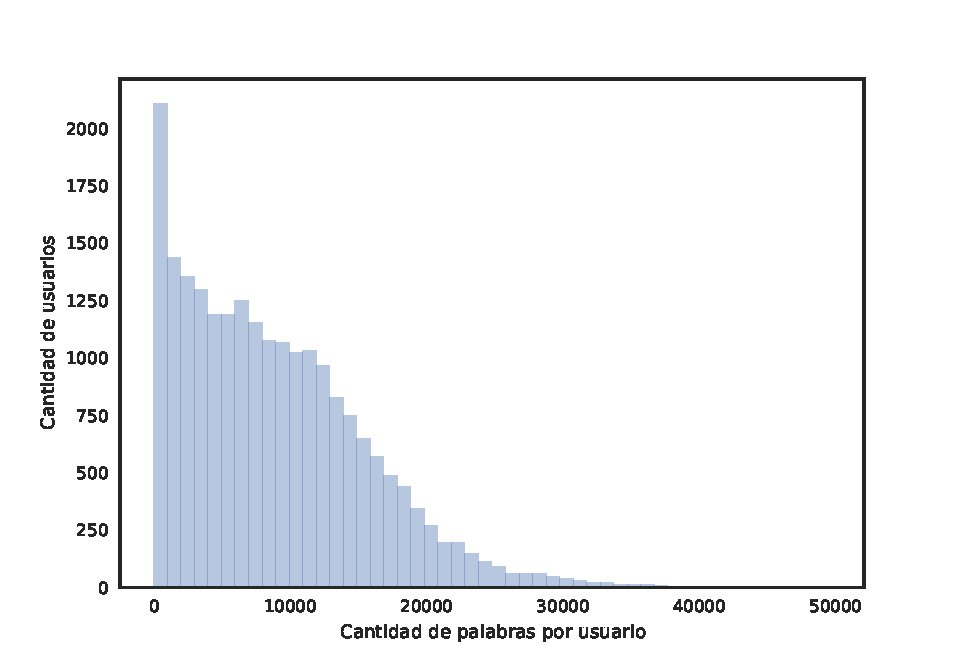
\includegraphics[width=\linewidth]{./images/train/conFiltro/cantPalabrasUsuario.pdf}
    \caption{Histograma de la cantidad de palabras totales por cada usuario (del conjunto de desarrollo).} 
    \label{fig:cantPalabrasUsuario} 
   \end{minipage}
   \begin{minipage}{0.49\textwidth}
    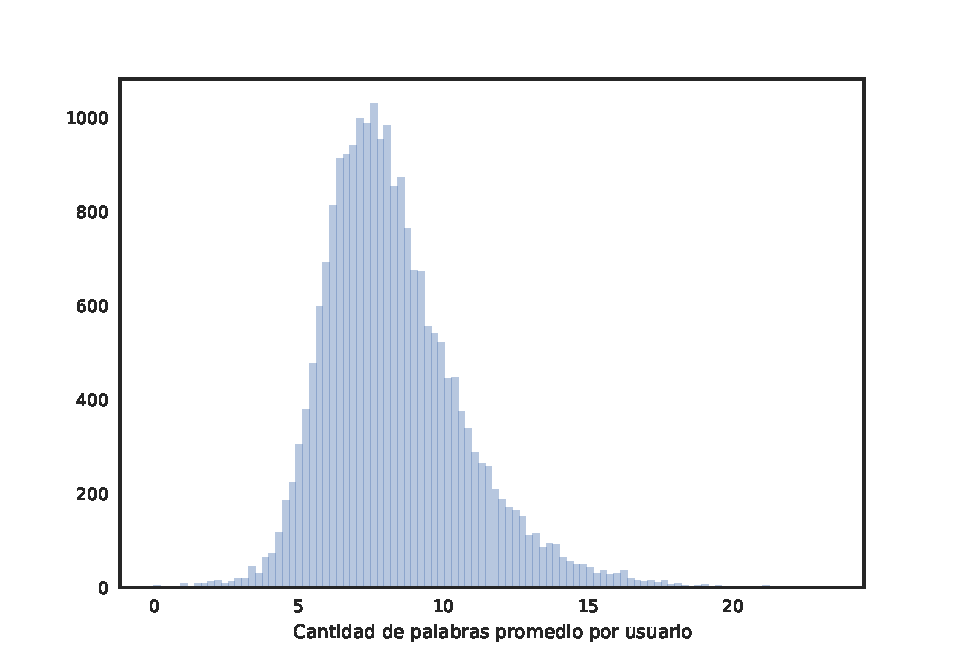
\includegraphics[width=\linewidth]{./images/train/conFiltro/cantPalabrasPromedio.pdf}
    \caption{Histograma de la cantidad de palabras promedio para todos los usuarios (del conjunto de desarrollo).} 
    \label{fig:cantPalabrasPromedio} 
   \end{minipage}
   
\end{figure}

%Cantidad de palabras promedio por tweet
%Cantidad de palabras por usuario + varianza por provincia
\subsection{Tuits a lo largo del tiempo}
Los tuits recolectados para el conjunto de datos de desarrollo tienen una particularidad: a medida que pasan los años 
hubo mayor cantidad de tuits durante un año. Esto se refleja en los gráficos de las figuras \ref{fig:histTweetsProvincia1} y \ref{fig:histTweetsProvincia2}.

\begin{figure}[!ht]\centering
   \begin{minipage}{0.49\textwidth}
     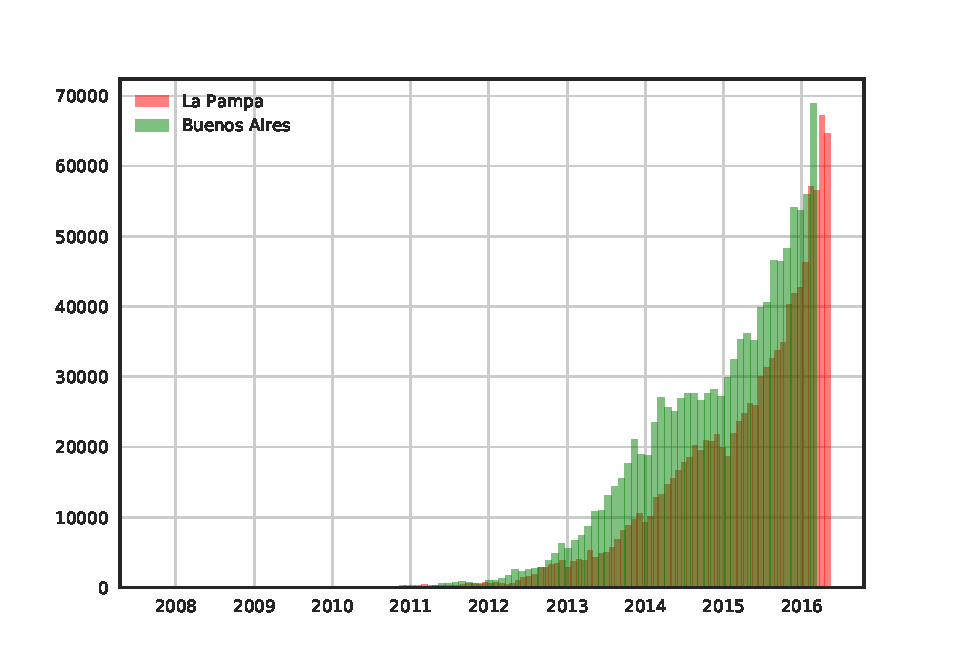
\includegraphics[width=\linewidth]{./images/train/sinFiltro/histTweetsProvincia1_sinFiltro.pdf}
     \caption{}
     \label{fig:histTweetsProvincia1}
   \end{minipage}
   \begin {minipage}{0.49\textwidth}
     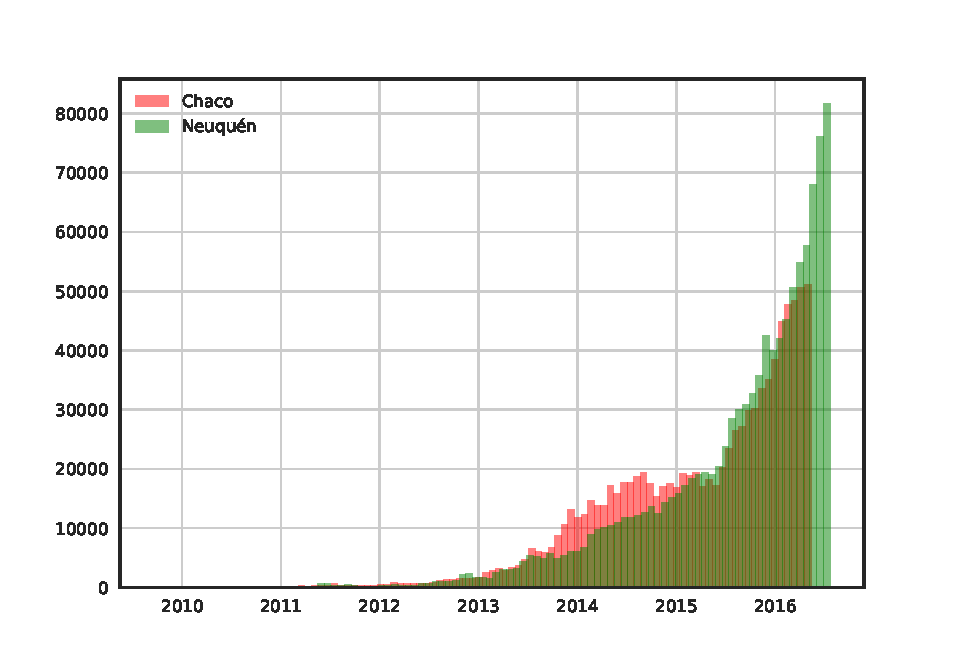
\includegraphics[width=\linewidth]{./images/train/sinFiltro/histTweetsProvincia2_sinFiltro.pdf}
     \caption{}
     \label{fig:histTweetsProvincia2}
   \end{minipage}
   \caption { En la figura \ref{fig:histTweetsProvincia1} se presenta un histograma donde se muestra la cantidad de tuits que se hicieron por intervalo de tiempo en la provincias La Pampa y Buenos Aires. En la figura \ref{fig:histTweetsProvincia2}, se presenta el gráfico para Chaco y Neuquén.}
\end{figure}


% Tweets promedio por usuario, por provincia. (varianza)

% cantidad de tweets por usuario, cantidad media de palabras por usuario

\section{Búsqueda de contrastes}

% Definir que es un contraste, que tiene un uso significativo en una region más que en otra. LAs alternativas que propusimos, z test binomial.
Una palabra tiene un contraste cuando esta tiene un uso con diferencias significativas en
distintas regiones. En este trabajo nos propusimos crear un listado con palabras con contrastes que tengan
importancia a nivel lingüístico. En este sentido, los nombres de personas, lugares u organizaciones no 
fueron considerados de interés a pesar de tener contrastes en su uso.
Este listado fue ordenado por una métrica que capte en un único valor el nivel contrastivo. De esta manera, 
se seleccionó un subconjunto de palabras, de acuerdo a la métrica, el cual fue analizado manualmente en otros textos por la Academia Argentina de Letras.

El primer acercamiento para ver el contraste de las palabras lo realizamos comparando las frecuencias de las palabras 
en cada par de provincias de la Argentina. Para esto calculamos, por cada palabra, la frecuencia de ocurrencias sobre cada una de las dos provincias. La mayor frecuencia de ambas, la llamamos frecuencia máxima y a la menor, la frecuencia mínima. Luego el cociente entre la frecuencia máxima y la frecuencia mínima tiene como resultado lo que llamamos \textit{maxDif}. En caso de que en una de las dos provincias no se haya 
recolectado tuits con esa palabra, se tomaba como frecuencia mínima a la frecuencia mínima distinta de 0 de todas las palabras generadas en esa provincia. Así se evitó la división por cero. Esta métrica se resumen en la ecuación \ref{eq:maxDif}.


\begin{equation}
  \label{eq:maxDif} 
  maxDif(w,prov_1,prov_2) = \frac{F_{max}(w,prov_1,prov_2)}{F_{Min}(w,prov_1,prov_2)}
\end{equation}
donde 
\begin{equation}
F_{max}(w) = \max(frec(w,prov_1),frec(w,prov_2))
\end{equation}

\begin{equation}
 F_{min}(w) = \left\{ \begin{array}{ll}
             \min(frec(w,prov_1),frec(w,prov_2))  \text{ si } frec(w,prov_1) > 0 \text{ y } frec(w,prov_2) > 0 & \\
             \\\min(frec(w,p)) \forall w \in palabras(p) , \text{ con } p=\{prov_1,prov_2\} \setminus \{P_{max}\} \text{sino} &  \\
             \end{array}
   \right.
\end{equation}
   donde $P_{max}$ es la provincia que tiene la mayor frecuencia de ambas.\\



De esa manera se ordenó el listado de cada par de provincias teniendo en cuenta la división de frecuencias. 
Sin embargo, este método imposibilitaba el trabajo manual para la Academia Argentina de Letras que debía mirar estos listados y hacer un análisis más exhaustivo sobre las palabras con mayor diferencia de frecuencias, debido a que había $\binom{23}{2} = 253$
listados (o equivalentemente 253 columnas en un mismo listado) a analizar. Además la métrica solo permitía saber si había un contraste entre dos provincias, pero no se podía tener en cuenta la frecuencia de la palabra en el resto de las provincias. 
% Mencionar que la idea era realizar un z test para obtener las palabras más significativas.
En consecuencia las palabras se encontraban repetidas en los distintos listados y con diferentes valores de \textit{maxDif}, lo cual hacía muy difícil poder identificar en que regiones había una diferencia significativa de frecuencias.

Debido a esto decidimos realizar un nuevo enfoque para encontrar las palabras con alta contrastividad en las distintas regiones, de manera que una métrica pueda reflejar el nivel de contrastividad de la palabra en un único valor.
De este modo, nos enfocamos en analizar el contraste de frecuencias de palabras sobre las provincias a través de una métrica superadora.

\subsection{Métricas para medir el contraste en la frecuencia de las palabras}
Dado que se quieren encontrar las palabras con contrastes significativos en distintas 
regiones se propone generar una métrica basada en la cantidad de información 
para poder realizar esta tarea.

Una medida que se puede usar para comparar las frecuencias de las palabras en las diferentes regiones del país puede ser la entropía definida por Shannon ( ver en el apéndice: \ref{sub:entropiaShannon}), debido a que podemos tener un valor que informe qué tan uniforme es la distribución de las frecuencias de cada palabra.
Sin embargo, la entropía como única medida tiene sus desventajas. Principalmente, una palabra con una sola ocurrencia en una provincia y ninguna en las demás, tiene la entropía mínima. A pesar de que nos interesan las palabras con un contraste significativo entre regiones, dentro de ellas elegiremos las que tienen mayor cantidad de ocurrencias. Es por esto que elaboramos otra métrica que tenga en cuenta la entropía, entre otras variables a tener en cuenta.


\subsection{Valor de información}
La métrica que utilizamos para ordenar los listados de palabras y detectar cuáles son
las que tienen altos contrastes en su uso en distintas regiones fue inspirada por el
trabajo de Zanette y Montemurro \cite{montemurro2010towards}.
Ellos, a diferencia de Shannon, estudiaron una relación entre una medida de la información y su función semántica en el lenguaje.
A continuación detallamos el procedimiento para calcular lo que ellos llamaron
el valor de la información:

Dado un texto dividido en P partes iguales, se calcula la entropía  $H(w)$ sobre el vector de cantidad de ocurrencias en cada una de las P ventanas.
Luego se define $\widehat{H(w)}$  como la entropía de una permutación aleatoria del texto y promediada por todos las posibles realizaciones de la permutación de él. 
%% CHEQUEAR LA DEFINICION DE LA ENTROPIA SHUFFLEADA

Es decir, se distribuyen uniformemente las palabras en P partes y se calcula la
entropía como se hizo con el texto original. Es de esperar que en la mayoría de casos 
la entropía del texto permutado sea mayor que la medida en el calculo original. Esto 
se debe a que las palabras se distribuyen de forma más uniforme 
en las distintas partes.

Finalmente, definen al valor de la información como $I(w) = p(w) (\widehat{\eta(w)} - \eta(w))$, con $p(w)$ la frecuencia total de la palabra en el texto. 
De esta manera se les da más importancia a las palabras que son más frecuentes y a las palabras que tienen una baja entropía, ya que en estas el término de la diferencia es más grande.

Este estudio se hizo sobre tres textos, \textit{Análisis de la mente}, 
\textit{Moby Dick} y \textit{El origen de las especies} de Charles Darwin. 
En los tres libros las palabras con mayor valor de la información están 
altamente relacionadas con los temas principales.

Si bien esta métrica tiene en cuenta la frecuencia de las palabras además de la 
entropía, el texto en Twitter resulta difícil de dividir en partes iguales. 
Esto es porque la división está pensada para dividir el texto en secciones que 
posiblemente hablen de distintos temas y nuestros textos son tuits que por lo general no superan las 10 palabras.
Otra dificultad que surge de esta métrica es la imposibilidad de realizar la media 
de todas las posibles permutaciones del texto por la limitación computacional ya que 
tenemos una cantidad muy grande de datos.

Es por eso que realizamos una métrica parecida:

Podemos pensar a las palabras del texto como una variable aleatoria W, donde cada palabra w tiene una probabilidad de aparición en una provincia dada de la Argentina. Esta probabilidad la aproximamos con la frecuencia en la que aparece, es decir la cantidad de ocurrencias de la palabra dividida por la cantidad de palabras totales.
Por otro lado sea P una variable aleatoria que cuenta la cantidad de personas que 
utilizan la palabra p en cada provincia.

Luego,
\begin{equation}
%I(w) =  norm_{p}(w) * norm_{u}(w) * (\widehat{H}_{w}(w) - H_{w}(w)) * (\widehat{H}_{p}(w) - H_{p}(w)) \\
I(w) =  I_p(w) * I_u(w)\\
\end{equation}
\begin{equation}
I_p(w) = norm_{p}(w) * (\widehat{H}_{w}(w) - H_{w}(w)) \\
\end{equation}
\begin{equation}
I_u(w) = norm_{u}(w) * (\widehat{H}_{u}(u) - H_{u}(w))
\end{equation}

\begin{equation}
norm_{p}(p) = \frac{cw(p)- MIN_W }{MAX_W - MIN_W}
\label{eq:norm1}
\end{equation}
donde:
\noindent\begin{minipage}{.5\linewidth}
\begin{equation}
  MIN_W = \min\limits_{p \in Palabras} cw(w)
\end{equation}
\end{minipage}%
\begin{minipage}{.5\linewidth}
\begin{equation}
  MAX_W = \max\limits_{p \in Palabras} cw(w)
\end{equation}
\end{minipage}
donde $cw(p)$ es igual al logaritmo sobre la cantidad de ocurrencias de esa palabra en toda la Argentina, es decir $cw(p) = \log_2(cantidadOcurrencias(p))$.

Análogamente,
\begin{equation}
norm_{u}(w) = \frac{cu(w)- MIN_U }{MAX_U - MIN_U}
\label{eq:norm2}
\end{equation}
\noindent\begin{minipage}{.5\linewidth}
\begin{equation}
  MIN_U = \min\limits_{p \in Palabras} cu(p)
\end{equation}
\end{minipage}%
\begin{minipage}{.5\linewidth}
\begin{equation}
  MAX_U = \max\limits_{p \in Palabras} cu(p)
\end{equation}
\end{minipage}
donde $cu(p)$ es el logaritmo sobre  la cantidad de usuarios que utilizan dicha palabra en la Argentina, es decir $cu(p)= \log_2(cantidadUsuarios(p)))$.
$\widehat{H}$ es la entropía con las cantidades distribuidas uniformemente y H es la entropía común.

Tanto $norm_{w}$ como $norm_{u}$ realizan una normalización del logaritmo de esas variables. Esto se debe a que el logaritmo genera una dispersión en las medidas de forma tal que su distribución sea más uniforme a lo largo de todo el rango de valores. Esto se puede ver en la figura \ref{fig:cantNorms}.
$\widehat{H}_{u}$ y $\widehat{H}_{w}$ se corresponde a las entropías de los vectores simulados de apariciones.
Esta simulación se realiza con una distribución multinomial ya que se distribuye la suma de los valores de la variable aleatoria uniformemente. 

% La variacion de la entropia se puede ver como una cantidad que mide cuanta información se necesita para poder obtener esa distribución
% Si las cantidades de ocurrencias (o de personas que utilizan) de un término están distribuidas uniformemente a través de todas las provincias, quiere decir que no aporta demasiada información 

\begin{figure}[!ht]
\centering
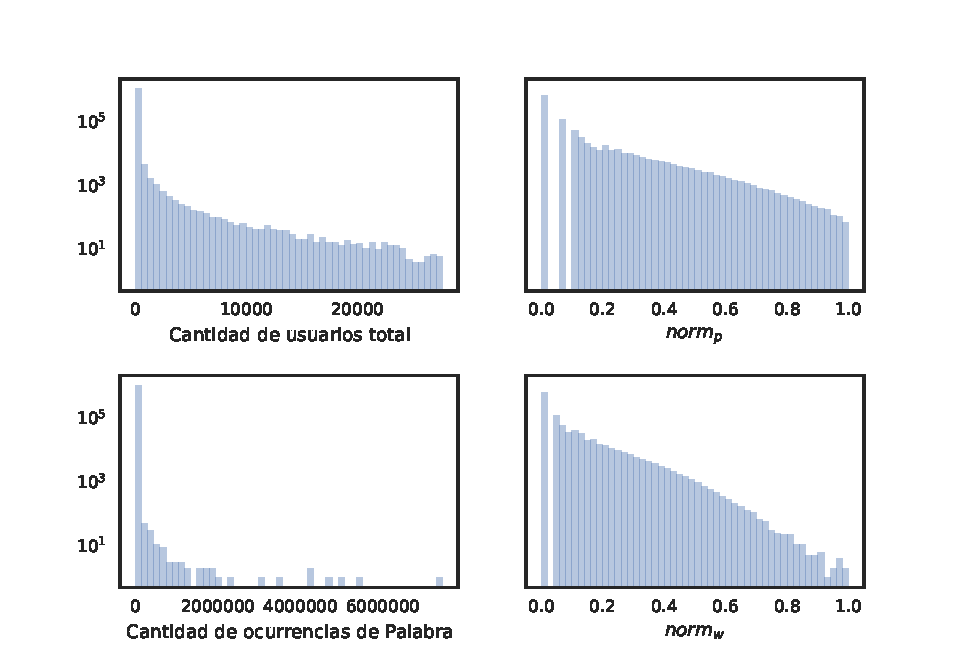
\includegraphics[width=1.0\textwidth]{./images/train/sinFiltro/cantNorms_sinFiltro.pdf}
\caption{Cantidades y sus normalizaciones: Mediante los histogramas presentamos la distribución de los valores de la cantidad de los usuarios totales que utilizaron cada palabra, como la cantidad de ocurrencias de una palabra. A la derecha se pueden observar la normalización de las variables descriptas en \ref{eq:norm1} y \ref{eq:norm2}.} 
\label{fig:cantNorms} 
\end{figure}

El término de la diferencia de la entropía sobre la cantidad de personas que utilizan la palabra tiene como objetivo mitigar el ruido de la entropía de palabras. En particular una determinada provincia o región pueden tener muchas ocurrencias de una palabra causado por algunos usuarios que utilizan constantemente el término. Un ejemplo de esto podrían ser bots que escriben automáticamente textos iguales (o similares) en grandes cantidades. Otra posible causa de este fenómeno podría ser la de usuarios de ciertas organizaciones que hablan de personas, lugares o marcas de forma constante.

Para eliminar los valores atípicos se procedió a remover las palabras que no superaran las 40 ocurrencias, como también aquellas que eran dichas por menos de 6 usuarios. 

\subsection{Frecuencia de las palabras}
\label{sub: frecuenciaPalabras}
% Ver si se hace este gráfico con todas las palabras ya que por ahora tengo el conjunto de palabras con más de 40 ocurrencias
En la figura \ref{fig:cantPalabras} graficamos la distribución de la cantidad de ocurrencias de las palabras.Podemos observar que la mayoría de las palabras ocurren poco. En particular el 50\% de las palabras ocurren menos de 139 veces. Por otro lado hay pocas palabras que ocurren mucho, por ejemplo la palabra \textit{que} o la preposición \textit{de}.

\begin{figure}[ht]
\centering
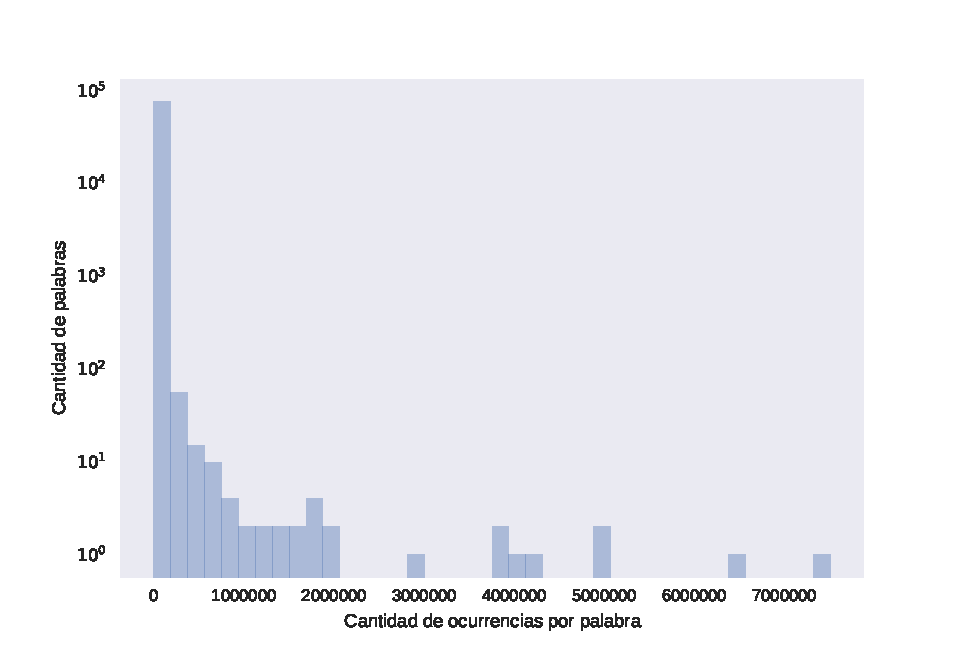
\includegraphics[width=0.8\textwidth]{./images/DistribucionOcurrenciasPalabras.pdf} 
\caption{Histograma de la cantidad de ocurrencias de las palabras} 
\label{fig:cantPalabras} 
\end{figure}

\begin{table}[ht]
\centering
\label{tab:palabrasMasOcurrentes}
\begin{tabular}{|c|c|}
\hline
Palabra & Cantidad de Ocurrencias \\ \hline
que     & 7509160                 \\
de      & 6527014                 \\
a       & 4962492                 \\
la      & 4913854                 \\
no      & 4177810                 \\
me      & 4101998                 \\
y       & 3838370                 \\
el      & 3773455                 \\
en      & 2969783                 \\
te      & 2060662                 \\
se      & 1976027                 \\
un      & 1863075                 \\
es      & 1825892                 \\
con     & 1799979                 \\
lo      & 1712189                 \\
mi      & 1643777                 \\
por     & 1553382                 \\
los     & 1498941                 \\
para    & 1398757                 \\
las     & 1212452                 \\
\hline
\end{tabular}
\caption{Cantidad de apariciones de las 20 palabras más frecuentes.}

\end{table}

Si comparamos la posición de la palabra en un listado ordenado podemos ver que se cumple con la ley de Zipf. Esta es una ley empírica formulada por George Zipf en el año 1932 en la cual se establece una relación entre la frecuencia de una palabra con su posición dentro del listado de palabras ordenadas por frecuencia decreciente. En particular, sea $n$ la posición de la palabra en el listado ordenado y sea $f(n)$ la cantidad de ocurrencias de la n-esima palabra, se puede hacer la siguiente aproximación:

$$f(n) \approx \frac{1}{n^{\alpha}}$$
donde $\alpha$ toma un valor levemente mayor a 1.
Entonces, bajo la ley de Zipf uno puede saber que la frecuencia de la segunda palabra más dicha en un corpus, es aproximadamente la mitad que la primera. La palabra con posición 3 en el listado ordenado por frecuencias, va a tener aproximadamente la tercera parte de la cantidad de ocurrencias que la primera y así sucesivamente. Otra forma de utilizar esta ley empírica es la siguiente:
sabiendo la posición de una palabra \textit{w} en el listado ordenado por frecuencias de un corpus A y sabiendo la cantidad de palabras totales de un corpus B, puede estimar la cantidad de ocurrencias de aquella palabra en el corpus B.
% HACER EJEMPLO
\begin{figure}[!ht]
\centering
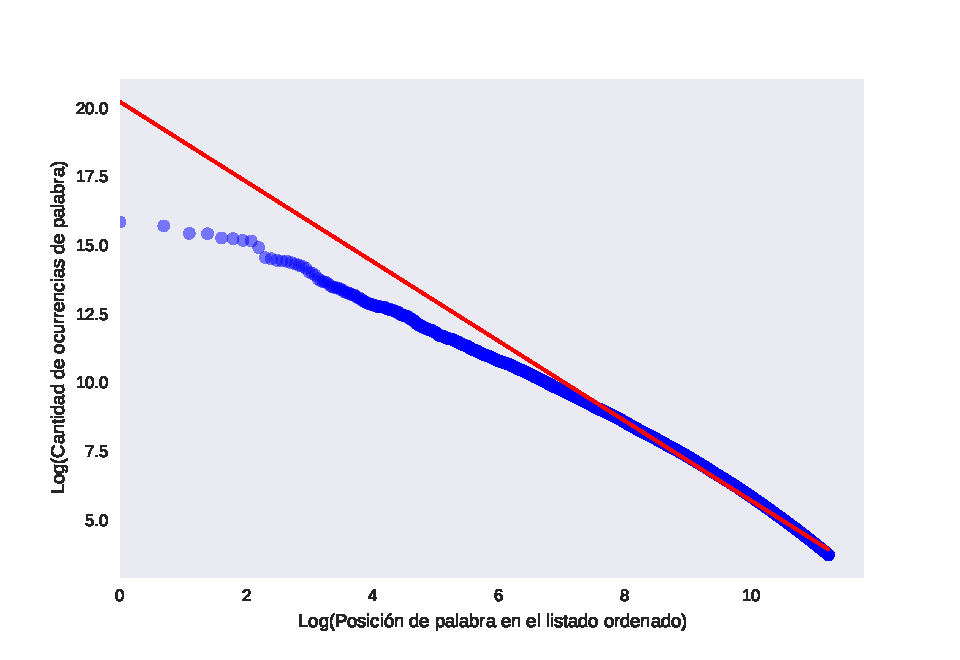
\includegraphics[width=0.5\textwidth]{./images/zipf.pdf}
\caption{Cantidad de Ocurrencias de palabra vs posición en listado ordenado. Se aplicó el logaritmo a las cantidades de ocurrencias, como también a los valores de las posiciones para mostrar la proporcionalidad entre $f(s)$ y $\frac{1}{s^{\alpha}}$.} 
\label{fig:zipf} 
\end{figure}


\subsection{Test Hipergeométrico}
Luego de realizar el listado de palabras ordenado por el valor de la información se aplicó un test estadístico para tener mayor confianza de que las palabras clasificadas como contrastivas realmente tienen esta propiedad y no fueron producto del azar. Se seleccionó un conjunto de palabras significativas a nivel lingüístico a partir de las 5000 palabras consideradas más contrastivas por nuestra métrica. 

Decidimos elegir el test hipergeométrico ya que queremos ver que la palabra sobre la que se hace el test no estuvo sobrerrepresentada en comparación con la población. Asumimos que la cantidad de ocurrencias de una palabra se puede modelar con una distribución hipergeométrica ya que se puede pensar como un experimento donde se obtuvieron k palabras exitosas en una región con n palabras y un total de N palabras en la Argentina. Las regiones que utilizamos para cada palabra son el conjunto de provincias que cubren el 80\% de las ocurrencias de dicho término. Luego, queremos calcular la significancia estadística de haber obtenido esas k palabras exitosas.

Luego, por cada palabra seleccionada como contrastiva le aplicamos el test estadístico con la siguiente hipótesis nula: la palabra tienen un uso homogéneo en las distintas regiones de la Argentina, es decir que la frecuencia de ocurrencias de cada palabra debería ser similar independientemente de la región.
Por lo tanto, en caso de que la palabra sea contrastiva deberíamos obtener una baja probabilidad de haber obtenido diferencias entre las frecuencias de la palabra en una región con el resto del país.  significativas sobre las frecuenciascomparandolas que la hipótesis nula no se cumple debido al azar.
% que la cantidad de ocurrencias de la palabra en la región elegida es mayor a lo observado. 
Por lo tanto, sea  cantPalabrasW(Region) igual a la cantidad de ocurrencias observada de la palabra en la región a analizar.


\begin{table}[ht]
\centering
\label{tab:contingencia}
\begin{tabular}{lccc}
\hline
& \#Palabras Sobre Region &\#Palabras en el resto de Argentina &Total \\ \hline
\# Palabras w &   k & K-k & K \\ 
\# Palabras $\neq$ w & n-k & N + k - n - K  & N - K \\ 
Total & n & N -n & N \\ \hline
\end{tabular}
\caption{Tabla de contingencia}

\end{table}



$$
\begin{cases}
H_0 :  x > cantPalabrasW(Region) \\
H_1 : x \leq cantPalabrasW(Region)
\end{cases}
$$  
siendo x la esperanza de la variable aleatoria que representa la cantidad de palabras exitosas en esa región.

% agregar gráficos de palabras comunes, con los parametros de la distribucion
% hacer un grafico de la distribución estimada (y la observada) de la cantidad de ocurrencias de la palabra 
Ante los p-valores tan bajos, decidimos hacer el test estadístico sobre palabras que consideramos que no tendían porque tener una frecuencia muy distinta en las distintas regiones. Realizamos el test para las palabras \{que, cuando, hola\} y estos también dieron p-valores menores a 0.001. Frente a esta situación investigamos las posibles causas de este fenómeno.

%Agregar lo de adam kilgariff